\section{I Codici Lineari a Blocco}
Fino ad ora abbiamo descritto i codici a blocco in modo generale, definendoli come un sottoinsieme $C$ di $M$ parole valide all'interno di uno spazio più ampio $q^n$. Tuttavia, affinché un codice sia implementabile tramite circuiti logici, deve possedere una struttura matematica rigorosa. Nasce così la famiglia più importante dei codici a blocco: i \textbf{Codici Lineari}.

\subsection{Definizione e Proprietà Fondamentali}
Un codice a blocco $C(n,k)$ su un alfabeto (\textit{campo}) con $q$ simboli si definisce \textbf{lineare} se le sue $M = q^k$ parole di codice formano un \textbf{sottospazio vettoriale} di dimensione $k$ all'interno dello spazio totale di dimensione $n$.
Di un codice lineare possiamo definire anche come parametro la distanza minima richiesta, con $C(n,k,d_{min})$.
\begin{itemize}
    \item $n$: lunghezza codeword
    \item $k$: dimensione (bit di informazione)
    \item $d_{min}$ distanza minima (\textit{la notazione può essere estesa per includere esplicitamente la distanza minima})
\end{itemize}
La \textit{linearità} garantisce proprietà molto importanti e \textit{utili}: la \textit{chiusura} rispetto alle operazioni di somma e prodotto.
\begin{itemize}
    \item la \textbf{somma} di due parole di codice è ancora una parola di codice
    \item il \textbf{prodotto} di una parola di codice per un elemento di $\mathcal{A}$ è ancora una parola di codice
    \item Una conseguenza della chiusura rispetto a somma e prodotto è il fatto che la codeword \textit{nulla}, composta solo di simboli $0$, deve far parte del codice
\end{itemize}

\begin{esempio}{Codice NON Lineare}
\[C=\{010,111\}\quad 010+111= 101 \notin C \implies \text{codice \textbf{non} lineare} \]
\end{esempio}

\begin{esempio}{Codice Lineare C(3,1)}
\[C=\{000,111\}\]
\begin{itemize}
\item \[000+111=111 \in C\]
\item \[000+000=000 \in C\]
\item \[111+111=000 \in C\]
\item \[000 \cdot 0 = 000 \in C \]
\item \[111 \cdot 0 = 000 \in C \]
\item \[000 \cdot 1 = 000 \in C \]
\item \[111 \cdot 1 = 111 \in C \]
\end{itemize}
$\implies C$ è un codice lineare.
\end{esempio}





\subsection{La Matrice Generatrice e la Codifica}
    % Slide 10-15: Costruzione di G con vettori base. L'operazione di codifica x = u * G.
    % Inseriamo qui il concetto di Codice Sistematico e la forma G = [I_k | A].
Poiché il codice costituisce un sottospazio vettoriale di dimensione $k$, lo si può definire tramite una \textbf{base} composta da \textbf{$k$ vettori linearmente indipendenti} di lunghezza $n$: $\vec{g}_1, \vec{g}_2, \dots, \vec{g}_k$.
Disponendo gli elementi della base come righe di una matrice, otteniamo la \textbf{matrice generatrice del codice} $G_{k \times n}$.
\begin{equation*}
G = 
\begin{pmatrix}
    g_{11} & g_{12} & \dots  & g_{1n} \\
    g_{21} & g_{22} & \dots  & g_{2n} \\
           & \vdots &        &        \\
    g_{k1} & g_{k2} & \dots  & g_{kn}
\end{pmatrix}
\end{equation*}
Il nome deriva dal fatto che, tramite combinazioni lineari tra righe, \textit{genera} parole di codice.
Permutando le righe, si ottiene un codice \textit{equivalente}.

\begin{esempio}{$C(5,1)$}
\[G=(1 \quad 1 \quad 1 \quad 1 \quad 1) \implies C=\{11111, 00000\}\]
Si tratta di un codice a ripetizione con $d_{min}=5$ che corregge fino a due errori.    
\end{esempio}
\begin{esempio}{$C(5,3)$}
\[G= \begin{pmatrix}
    1 & 1 & 1 & 0 & 0\\
    0 & 0 & 1 & 1 & 0\\
    1 & 1 & 1 & 1 & 1\\
\end{pmatrix}
\]
Le parole di codice sono $q^k= 2^3=8$:
\[00000 \space 11100 \space 00110  \space 11111\]
\[11010 \space 00011 \space 11001  \space 00101\]
La distanza minima è $d_{min}=2$, quindi il codice può rilevare errori di peso $d_{min}-1=1$, e non può correggere alcuna configurazione di errore di peso 1 (per farlo servirebbe $d_{min}=3$).
\end{esempio}

\begin{esempio}{$C(7,4)$}
\begin{center} 
        \begin{equation*}
        G = 
        \begin{pNiceMatrix}[
            margin,
            code-before = { \rectanglecolor{blue!15}{1-1}{4-4} }
        ]
            1 & 0 & 0 & 0 & 0 & 1 & 1 \\
            0 & 1 & 0 & 0 & 1 & 0 & 1 \\
            0 & 0 & 1 & 0 & 1 & 1 & 0 \\
            0 & 0 & 0 & 1 & 1 & 1 & 1 
        \end{pNiceMatrix}
        \end{equation*}

        \vspace{-0.5em}
        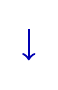
\begin{tikzpicture}[blue!70!black, thick]
            \draw[->] (0,0.4) -- (0,0);
        \end{tikzpicture} \\
        \small \textit{Sottomatrice di rango 4 (Identità $I_4$)}
    \end{center}
Le parole di codice sono $q^k=2^4 =16$. La matrice $G$ in questo caso ha una forma particolare, $([I_k \mid A])$.
\end{esempio}

\subsubsection{Matrice Sistematica}
Se la matrice generatrice è della forma $([I_k \mid A])$, con $I_k$ la \textit{matrice identità} di ordine $k$, e $A_{k \times (n-k)}$, allora si dice \textbf{sistematica} o \textbf{in forma canonica}. La \textit{sistematicità} implica che, a seguito della codifica, i primi $k$ bit delle codeword saranno identici ai bit del messaggio originale (il \textit{payload} lungo $k$). Questo rende l'estrazione dell'informazione una operazione banale per il ricevitore.

\subsection{Codifica di un codice Lineare}
Le proprietà dei codici lineari semplificano il processo di codifica dei dati; si riduce la codifica a un prodotto tra vettore (dato in ingresso) e matrice (la matrice generatrice).
Per codificare un vettore in ingresso $u=\langle u_1,\dots,u_k \rangle$ in una parola di codice $x=\langle x_1,\dots,x_n\rangle$ si calcola
\[x=u \cdot G\]
Questo corrisponde a una trasformazione lineare da uno spazio di dimensione $k$ a uno di dimensione $n$. Così viene \textit{aggiunta} la \textbf{ridondanza} necessaria per correggere gli errori.

\begin{esempio}{$C(5,3)$}
Riprendiamo la matrice generatrice $G_{3 \times 5}$ vista in precedenza:
\[G= \begin{pmatrix}
    1 & 1 & 1 & 0 & 0\\
    0 & 0 & 1 & 1 & 0\\
    1 & 1 & 1 & 1 & 1\\
\end{pmatrix}\]
Per codificare il messaggio $u=<u_1,u_2,u_3>$ si calcola

\begin{align*}
    x &= u \cdot G = \\
      &= (u_1, u_2, u_3) \cdot 
    \begin{pmatrix}
        1 & 1 & 1 & 0 & 0 \\
        0 & 0 & 1 & 1 & 0 \\
        1 & 1 & 1 & 1 & 1 \\
    \end{pmatrix} = \\
      &= (u_1 + u_3, \space u_1 + u_3, \space u_1 + u_2 + u_3, \space u_2 + u_3, \space u_3)
\end{align*}
\begin{itemize}
    \item $u=101 \implies 00011$
    \item $u=001 \implies 11111$
\end{itemize}
\end{esempio}

\begin{esempio}{Codifica in forma sistematica $C(7,4)$}
\begin{equation*}
G = 
\begin{pNiceMatrix}[
    margin,
    % Colorazione dello sfondo applicata prima del testo
    code-before = {
        \rectanglecolor{blue!15}{1-1}{4-4}   % Sottomatrice I4
        \rectanglecolor{yellow!15}{1-5}{4-7} % Sottomatrice P
    }
]
    1 & 0 & 0 & 0 & 0 & 1 & 1 \\
    0 & 1 & 0 & 0 & 1 & 0 & 1 \\
    0 & 0 & 1 & 0 & 1 & 1 & 0 \\
    0 & 0 & 0 & 1 & 1 & 1 & 1 
\end{pNiceMatrix}
\end{equation*}

% Definizione colori coerenti con la matrice G
\definecolor{info}{HTML}{E3F2FD}    % Azzurro chiaro
\definecolor{control}{HTML}{FFF9C4} % Giallo chiaro

\begin{equation*}
    x = (u_1, u_2, u_3, u_4) \cdot G = 
    ( \colorbox{info}{$u_1, u_2, u_3, u_4$} , \space
      \colorbox{control}{$u_2+u_3+u_4, u_1+u_3+u_4, u_1+u_2+u_4$} )
\end{equation*}

% Legenda centrata sotto l'equazione
\begin{center}
    \small
    \colorbox{info}{\phantom{x}} $k$ simboli informativi \quad
    \colorbox{control}{\phantom{x}} $n-k$ simboli di controllo
\end{center}
Ad esempio con $u= \langle1010\rangle$, $x= u \cdot G = \langle1010101\rangle$.
\end{esempio}





\subsection{La Matrice di Controllo della Parità (H)}
Fino ad ora abbiamo analizzato il codice dal punto di vista del trasmettitore; la matrice generatrice $G$ è lo strumento per mappare un messaggio in una parola di codice valida $\vec{x}$. Ora analizziamo il problema inverso: come si sfruttano le proprietà algebriche dei codici lineari per stabilire se la sequenza $\vec{y}$ in uscita dal canale corrisponde a una parola del codice $C$ \textit{legittima} o se è stata corrotta da un errore?

La linearità ci permette di definire un \textbf{test di validità algebrico} e ci evita un confronto sistematico di $\vec{y}$ con l'intero dizionario del codice. La decodifica ci permetterà quindi di riconoscere messaggi validi, o di identificare e in certi casi correggere eventuali errori.
Per realizzare la decodifica serve introdurre il concetto di codice duale derivante dagli spazi ortogonali.

\subsubsection{Codice Duale}
Dato un codice lineare $C(n,k)$, definiamo il suo \textbf{sottospazio ortogonale} (o \textbf{Codice Duale}) $C^\perp$, come l'insieme dei vettori di $\mathcal{A}^n$ ortogonali a tutte le parole di $C$:

\begin{align*}
C^\perp(n,k) &= \{y \space\colon \space y \perp x, \forall x \in C\} \\
             &= \{ y \space \colon \space y \cdot x^T = 0, \textit{ per ogni parola di codice} \}
\end{align*}

Dall'algebra lineare, essendo il codice $C$ un \textbf{sottospazio vettoriale} di dimensione $k$, esisterà sempre uno spazio ad esso \textbf{\textit{ortogonale}} di dimensioni $n-k$. I vettori di questo sottospazio $C^\perp$ godono di una proprietà importante: un vettore $y$ farà parte di $C^\perp$ se  il suo prodotto scalare con qualsiasi vettore di $C$ (quindi qualsiasi parola di codice) restituisce esattamente lo scalare \textbf{zero}.
Da questa proprietà algebrica si deriva la relazione detta \textbf{equazione di controllo} che, nei fatti, ai nostri fini realizza il controllo di validità sui messaggi ricevuti dal canale:

\[x_1 \cdot y_1 + x_2 \cdot y_2 + \dots + x_n \cdot y_n = 0\]
Si deduce che un codice $C(n,k)$ avrà $s^{n-k}$ equazioni di controllo.


\subsubsection{Il Codice Duale e la Matrice H}
    % Slides 16-19, 24-25: Definizione di spazio ortogonale. H * x^T = 0.
    % Costruzione rapida di H per codici sistematici: H = [-A^T | I_{n-k}].
Il codice duale $C^\perp$ è composto da $n-k$ vettori linearmente indipendenti, che generano il codice duale stesso; sono quindi una \textbf{base} per $C^\perp$. 
Raggruppando \textit{per righe} i vettori di questa base, otteniamo la \textbf{Matrice di Controllo della Parità di $C$} $\mathbf{H}$, che avrà quindi dimensioni $(n-k) \times n$.
\begin{equation*}
H = 
\begin{pmatrix}
    h_{11} & h_{12} & \dots  & h_{1n} \\
    h_{21} & h_{22} & \dots  & h_{2n} \\
           & \vdots & \dots  &        \\
    h_{(n-k)1} & h_{(n-k)2} & \dots  & h_{(n-k)n}
\end{pmatrix}
\end{equation*}
Essendo costruita con i vettori dello spazio ortogonale $C^\perp$, $H$ condensa in un'unica equazione matriciale tutte le equazioni di controllo. Quindi, se $\vec{x}$ è una parola di codice, vale l'equazione:
\begin{equation*}
H \cdot x^T = 
\begin{pmatrix}
    h_{11} & h_{12} & \dots  & h_{1n} \\
    h_{21} & h_{22} & \dots  & h_{2n} \\
           & \vdots &        &        \\
    h_{(n-k)1} & h_{(n-k)2} & \dots  & h_{(n-k)n}
\end{pmatrix}
\begin{pmatrix}
    x_1 \\
    x_2 \\
    \vdots \\
    x_n
\end{pmatrix} = 
\begin{pmatrix}
    0 \\
    0 \\
    \vdots \\
    0
\end{pmatrix}
\end{equation*}
Se $x$ non è una parola di codice, si avrà invece che:
\[H \cdot x^T \neq 0 \implies x \notin C \implies \vec{x} = \vec{z}+ \vec{w} \quad (z \in C, w \in C^\perp)\]

\paragraph{Matrice di controllo in forma canonica}
Se la matrice generatrice $G$ è in forma canonica ($G = [I_k \mid A]$), conseguentemente anche $H$ si costruisce in forma sistematica:
\[H= [-A^T | I_{n-k}]_{n-k \times n}\]
Questa costruzione non è casuale; è l'unica che garantisce la proprietà fondamentale $G \cdot H^T = 0$.
Possiamo fare delle osservazioni:
\begin{itemize}
    \item $H$ ha rango $n-k$
    \item In un campo $GF(2)$, lavoriamo in aritmetica \textit{modulo 2} (dove $-1 \equiv 1$), quindi il segno meno di $-A^T$ nei fatti \textit{sparisce}, ottenendo $H= [A^T \mid I_{n-k}]$.
    \item $\forall x  \in C, \space H \cdot x^T=0$
\end{itemize}

Ricapitolando: ogni messaggio $u$ di $k$ bit viene codificato in una parola di codice $x$ tramite l'operazione $x= u \cdot G$; quindi, per come abbiamo costruito le matrici $G$ ed $H$, vale la relazione $H \cdot x^T=0$ che definisce ogni codeword \textbf{valida}. Infatti:
\[x^T = G^T \cdot u^T \implies H \cdot x^T= H \cdot G^T \cdot u^T \implies H \cdot x^T=\vec{0}_{n-k}\]
Questo poiché, per costruzione, sappiamo che $H \cdot G^T = \mathbf{0}$.



\subsubsection{Matrice di Controllo e Distanza Minima}
    % Slides 20-21, 26-28: Questo è un teorema cruciale per l'orale! 
    % d_min corrisponde al numero minimo di colonne di H linearmente dipendenti.
I vincoli nella costruzione di $H$ consentono di utilizzarla per inferire la distanza minima del codice. Scrivendo $H$ \textit{per colonne}, $H=[\vec{h_1} \mid \vec{h_2} \mid \dots \mid \vec{h_n}]$, si può riscrivere il prodotto $H \cdot x^T$, il \textit{controllo di correttezza di $x$}, come somma di colonne:
\[\sum_{i=1}^n x_i \cdot \vec{h_i}\]
Il numero di colonne effettivamente sommate dipende dal numero di bit di $x$ di valore $1$, cioè dal \textbf{peso} $wt(x)$.
Poiché una parola $x$ appartiene a $C$ se e solo se questa somma dà come risultato il \textbf{vettore nullo} ($\mathbf{0}$), stiamo di fatto sommando tra loro esattamente $wt(x)$ colonne della matrice. Per i principi dell'algebra lineare, se la somma di $wt(x)$ colonne (con $wt(x) > 0$) dà il vettore nullo, significa per definizione che quelle $wt(x)$ colonne sono \textbf{linearmente dipendenti} tra loro.
Viceversa, per ogni combinazione lineare nulla di $w$ colonne di $H$, esiste una parola $x'$ tale per cui $wt(x')=w$.

Il legame tra il peso delle parole e le colonne di $H$ fornisce lo strumento per calcolare la prestazione principale del codice: la sua \textbf{distanza minima} ($d_{min}$).
Il nesso logico si basa sulla proprietà di linearità:
\begin{itemize}
    \item La distanza di Hamming tra due parole di codice qualsiasi $x$ e $y$ equivale al peso della loro differenza (o somma, in modulo 2): $d(x,y) = wt(x+y)$.
    \item Poiché il codice è lineare, la somma di due parole di codice genera \textit{sempre} un'altra parola di codice valida $z \in C$. Quindi: $d(x,y) = wt(z)$.
\end{itemize}

La distanza minima tra due parole equivale quindi a cercare la singola parola di codice (diversa da quella nulla) con il peso minore in assoluto. Si giunge così all'equivalenza fondamentale per i codici lineari:
\[ d_{min} = \min_{x,y\in C,x \neq y}{d_H(x,y)}=\min_{x'\in C,x' \neq 0}{d_H(x',0)} = \min_{x'\in C,x' \neq 0}{wt(x')} \]
\textit{La distanza minima di un codice lineare coincide con il peso minimo delle sue parole diverse da zero.}

Questa equivalenza e quanto dimostrato in precedenza sulle colonne di $H$, portano ad  enunciare il teorema finale:
se la parola valida più "leggera" del codice ha peso $w_{min}$, significa che il numero più piccolo di colonne di $H$ che sommate danno il vettore nullo è esattamente $w_{min}$.
Di conseguenza:
\[ d_{min} = \text{numero minimo di colonne di } H \text{ linearmente dipendenti} \]

\subsubsection{Proprietà dei codici lineari a blocchi (sistematici)}
Ricapitoliamo le proprietà fondamentali dei codici lineari a blocchi:
\begin{enumerate}
    \item Il codice a blocchi è costituito dalla parola nulla (tutti zeri) e da tutte le possibili combinazioni lineari (somme) delle righe della matrice generatrice $G$.
    \item La distanza di Hamming minima $d_{min}$ coincide con il peso minimo delle codeword diverse dalla parola nulla.
    \item \textbf{Distribuzione dei pesi}: è l'elenco di tutti i possibili pesi assunti dalle parole del codice, associato al numero di parole che possiedono ciascun peso.
    \item \textbf{Codici equivalenti}: due codici si dicono equivalenti se le loro matrici generatrici ($G$ e $G'$) sono ottenibili l'una dall'altra tramite operazioni elementari sulle righe e permutazioni sulle colonne.
    \item Due codici equivalenti condividono le stesse prestazioni a livello di blocco: hanno la stessa distribuzione dei pesi e la stessa probabilità di individuare una parola errata.
    \item Tuttavia, a parità di canale, due codici equivalenti avranno \textit{probabilità di errore sui singoli bit} diverse, poiché utilizzano una diversa mappatura tra messaggio e codeword (i codificatori sono diversi).
    \item \textbf{Teorema di equivalenza}: ogni codice lineare a blocchi $(n,k)$ non sistematico è sempre equivalente a un codice lineare a blocchi $(n,k)$ in forma sistematica.
\end{enumerate}

Per i codici che si presentano in forma \textbf{sistematica}, valgono in aggiunta le seguenti proprietà:
\begin{enumerate}
    \item La matrice generatrice è sempre riconducibile alla forma \textit{canonica} $G = [I_k \mid A]$.
    \item Nel caso binario, i primi $k$ bit della parola coincidono esattamente con i bit del messaggio, mentre i rimanenti $n-k$ sono i bit di controllo (o di parità).
    \item una parola di codice sistematico può essere indicata in due modi:
    \[u=(\textcolor{blue}{u_1,\dots,u_k}) \quad x=(\textcolor{blue}{u_1,\dots,u_k},\textcolor{red}{x_{k+1},\dots,x_n})\]
\end{enumerate}

\begin{esempio}{Esempio in forma sistematica}
\[\mathcal{A}=\{0,1\},C=(7,4)\]
\begin{center}
\renewcommand{\arraystretch}{1.3}
\begin{equation*}
% --- MATRICE G ---
G = 
\begin{pNiceMatrix}[
    margin,
    % Colorazione sottomatrici
    code-before = {
        \rectanglecolor{blue!15}{1-1}{4-4}   % I4 (Blu)
        \rectanglecolor{yellow!15}{1-5}{4-7} % A  (Giallo)
    },
    % Etichette inferiori centrate sotto i blocchi
    code-after = {
        \begin{tikzpicture}
            \node [below=10pt] at (4-2.5) {$I_4$};
            \node [below=10pt] at (4-6) {$A$};
        \end{tikzpicture}
    }
]
    1 & 0 & 0 & 0 & 0 & 1 & 1 \\
    0 & 1 & 0 & 0 & 1 & 0 & 1 \\
    0 & 0 & 1 & 0 & 1 & 1 & 0 \\
    0 & 0 & 0 & 1 & 1 & 1 & 1 
\end{pNiceMatrix}
\qquad \quad % Spazio tra le due matrici
% --- MATRICE H ---
H = 
\begin{pNiceMatrix}[
    margin,
    % Colorazione sottomatrici (Invertita rispetto a G)
    code-before = {
        \rectanglecolor{yellow!15}{1-1}{3-4} % -A^T (Giallo)
        \rectanglecolor{blue!15}{1-5}{3-7}   % I3   (Blu)
    },
    % Etichette inferiori centrate sotto i blocchi
    code-after = {
        \begin{tikzpicture}
            \node [below=10pt] at (3-2.5) {$-A^T$};
            \node [below=10pt] at (3-6) {$I_3$};
        \end{tikzpicture}
    }
]
    0 & 1 & 1 & 1 & 1 & 0 & 0 \\
    1 & 0 & 1 & 1 & 0 & 1 & 0 \\
    1 & 1 & 0 & 1 & 0 & 0 & 1
\end{pNiceMatrix}
\end{equation*}
\end{center}   
Applicando il teorema precedente alla matrice di controllo $H$ possiamo dedurre la distanza minima del codice in modo puramente \textit{visivo}:
\begin{itemize}
    \item Il peso minimo \textbf{NON} può essere $1$: servirebbe una singola colonna $\vec{h_i}$ linearmente dipendente da sola, il che implica che $\vec{h_i} = \mathbf{0}$; guardando $H$, non ci sono colonne nulle
    \item Il peso minimo \textbf{NON} può essere $2$: servirebbero due colonne che sommate danno zero ($\vec{h_i} + \vec{h_j} = \mathbf{0}$). In aritmetica modulo 2, questo accade solo se $\vec{h_i} = \vec{h_j}$. Guardando $H$, non esistono due colonne identiche.
    \item Il peso minimo \textbf{PUÒ} essere $3$: è infatti facile trovare combinazioni di tre colonne che sommate in modulo 2 si annullano (es. le prime tre colonne: $\vec{h_1}+\vec{h_2}+\vec{h_3} = \mathbf{0}$).
    \item è un esempio di codice di Hamming
\end{itemize}


\end{esempio}

\subsection{Decodifica Algebrica: Sindrome e Tabella di Slepian}
La codifica aggiunge ridondanza \textit{strutturata} al messaggio originale; nella trasmissione il canale rumoroso \textit{può aggiungere} una quota di rumore, alterando i bit in ingresso al canale. La decodifica ha quindi il duplice compito di \textbf{rivelare} se il rumore ha modificato il messaggio e, nei limiti delle capacità del codice, \textbf{correggerlo}.
In termini vettoriali, il modello del canale introduce un \textbf{vettore d'errore} $\vec{e}$ (che presenta degli "1" in corrispondenza delle posizioni alterate dal rumore). La sequenza ricevuta $\vec{y}$ sarà quindi:

\begin{center}

\resizebox{\textwidth}{!}{
    \begin{tikzpicture}[
        node distance=1.2cm,
        block/.style={rectangle, draw, fill=blue!15, text width=2.2cm, align=center, minimum height=1.2cm, thick, rounded corners=2pt},
        sum/.style={circle, draw, fill=gray!10, minimum size=6mm, thick, inner sep=0pt},
        arrow/.style={-Stealth, thick},
        label_txt/.style={font=\small\itshape, align=center, color=red}
    ]

        % Nodi principali
        \node (input) {$\vec{u} = (u_1, \dots, u_k)$};
        
        \node [block, right=of input] (cc) {Codifica di \\ Canale (CC)};
        
        \node [right=of cc] (x) {$\vec{x} = (x_1, \dots, x_n)$};
        
        % Etichetta "parola trasmessa" sopra il vettore x
        \node [above=0.3cm of x, label_txt] {parola \\ trasmessa};
        
        \node [block, right=of x] (chan) {Canale};
        
        % Nodo Somma per il Rumore (XOR)
        \node [sum, right=of chan] (plus) {$+$};
        
        % Nodo Rumore (Input superiore)
        \node [above=0.8cm of plus, color=red, font=\bfseries] (noise) {$\vec{e}$ (Rumore)};
        
        % Sequenza ricevuta
        \node [ellipse, draw, fill=red!10, right=of plus, minimum height=1cm, align=center] (y) {$\vec{y} = (y_1, \dots, y_n)$ \\ \small seq. ricevuta};

        % Connessioni
        \draw [arrow] (input) -- (cc);
        \draw [arrow] (cc) -- (x);
        \draw [arrow] (x) -- (chan);
        \draw [arrow] (chan) -- (plus);
        \draw [arrow, color=red] (noise) -- (plus);
        \draw [arrow] (plus) -- (y);

    \end{tikzpicture}
}
\end{center}

Da cui il vettore di errore risulta matematicamente definito come la differenza (equivalente alla somma in aritmetica modulo 2) tra il vettore ricevuto e la parola originariamente trasmessa:
\[ \vec{e} = \vec{y} - \vec{x} \quad (\text{ovvero } \vec{e} = \vec{y} + \vec{x} \text{ in } GF(2)) \]
Tuttavia, il decodificatore conosce \textit{esclusivamente} la sequenza ricevuta $\vec{y}$. Non conoscendo né la parola corretta $\vec{x}$ né l'errore $\vec{e}$, l'equazione appena scritta non è direttamente risolvibile.
Serve un ulteriore oggetto matematico per risolvere il problema, la \textbf{sindrome di $y$}. in grado di analizzare $\vec{y}$, "filtrare via" l'incognita $\vec{x}$ e far emergere solo le informazioni relative all'errore $\vec{e}$. Questo strumento è la chiave della decodifica algebrica e si basa sull'uso della matrice di controllo $H$.

\subsubsection{Il Vettore Sindrome}
Si definisce \textbf{sindrome di $y$} il vettore ottenuto moltiplicando la matrice di controllo $H$ per il trasposto del vettore ricevuto dal canale:
\[ S(y) = H \cdot y^T \]
In questa fase, $H$ \textit{adempie} alla sua funzione di \textbf{controllo}: i singoli zeri presenti nel vettore sindrome corrispondono alle equazioni di parità che sono state soddisfatte. Pertanto:
\[ S(y) = \mathbf{0} \iff y \in C \iff x+e \in C \]
La sindrome ha dimensione $n-k$, pari al numero di equazioni di controllo.
Una proprietà fondamentale è che la sequenza ricevuta $y$ e il vettore di errore $e$ hanno la \textbf{stessa sindrome}. Infatti, poiché $x$ è una parola di codice valida ($H \cdot x^T = \mathbf{0}$), si ha:
\[ S(y) = H \cdot y^T = H \cdot (x^T+e^T) = H\cdot x^T + H \cdot e^T = \mathbf{0} + H \cdot e^T = S(e) \]

La sindrome, come suggerisce il nome medico, \textit{diagnostica} la presenza e la configurazione dell'errore. Dipendendo esclusivamente da quest'ultimo ($S(y) = S(e)$), permette di "isolare" l'errore dal messaggio trasmesso, ignorando $x$, per cercare, se possibile, di correggerlo.

\paragraph{Rivelazione di errori tramite Sindrome}
Sfruttando le proprietà appena definite, il processo di decodifica \textbf{algebrica} si articola in una sequenza di passi:
\begin{enumerate}
    \item \textbf{Calcolo:} Ricevuto il vettore $y$, il decodificatore calcola la sindrome $S(y) = H \cdot y^T$.
    \item \textbf{Rivelazione:} Si verifica il valore di $S(y)$:
    \begin{itemize}
        \item Se $S(y) = \mathbf{0}$, si assume che non si siano verificati errori (o che si sia verificato un errore non rilevabile). La parola viene accettata così com'è: la stima della parola trasmessa è $\hat{x} = y$.
        \item Se $S(y) \neq \mathbf{0}$, viene rilevato un errore.
    \end{itemize}
    \item \textbf{Correzione (se necessaria):} Una volta rilevato l'errore, si procede a stimarne la configurazione più probabile per poter correggere la parola ricevuta.
\end{enumerate}


\subsection{Correzione di errori tramite Sindrome e Tabella di Slepian}

Per poter correggere un errore, il ricevitore deve associare la sindrome calcolata $S(y)$ al vettore d'errore $\vec{e}$ che l'ha generata. Tuttavia, sorge un problema pratico: a una singola sindrome corrispondono esattamente $s^k$ vettori di errore possibili.

Data un'ipotetica configurazione di errore $\vec{e}$, se la sommiamo a una qualsiasi parola di codice $\vec{x}_i \in C$ (con $1 \leq i \leq s^k$), la linearità della sindrome porta a:
\[ S(x_i + e) = S(x_i) + S(e) = \mathbf{0} + S(e) = S(e) \]
Questo dimostra che esistono esattamente $s^k$ sequenze diverse che condividono la \textbf{stessa identica sindrome}. Quando il ricevitore ottiene $S(y)$, ha quindi $s^k$ "candidati" possibili per l'errore. Come sceglie quello giusto?

Si partiziona l'intero spazio vettoriale delle sequenze ricevibili ($\mathcal{A}^n$) costruendo la \textbf{Tabella Standard di Slepian} (o \textit{Standard Array}).

La tabella distribuisce le $s^n$ possibili sequenze ricevibili in una griglia strutturata in questo modo:
\begin{itemize}
    \item La tabella è costituita da \textbf{$s^{n-k}$ righe}, tante quante sono le possibili configurazioni della sindrome.
    \item Ogni riga contiene \textbf{$s^k$ elementi} (colonne), tutti accomunati dall'avere la stessa sindrome. In algebra, ciascuna di queste righe prende il nome di \textbf{classe laterale} (o \textit{coset}) del sottogruppo $C$.
    \item \textbf{La prima riga} (quella associata alla sindrome nulla $\mathbf{0}$) contiene esattamente le $s^k$ parole di codice valide $\vec{x}_i \in C$.
\end{itemize}

\definecolor{rowblue}{HTML}{E3F2FD}
\definecolor{headerblue}{HTML}{1565C0}

\begin{center}
\renewcommand{\arraystretch}{1.5}
\small
% --- TABELLA STANDARD GENERICA ---
\begin{tabular}{|c|c|c|c|c|}
    \hline
    \rowcolor{white} $\vec{x}_0 = \vec{e}_0 = (0, \dots, 0)$ & $\vec{x}_1$ & $\vec{x}_2$ & $\dots$ & $\vec{x}_{2^k-1}$ \\ \hline
    \rowcolor{rowblue} $\vec{e}_1$ & $\vec{x}_1 + \vec{e}_1$ & $\vec{x}_2 + \vec{e}_1$ & $\dots$ & $\vec{x}_{2^k-1} + \vec{e}_1$ \\ \hline
    \rowcolor{white} $\vec{e}_2$ & $\vec{x}_1 + \vec{e}_2$ & $\vec{x}_2 + \vec{e}_2$ & $\dots$ & $\vec{x}_{2^k-1} + \vec{e}_2$ \\ \hline
    \rowcolor{rowblue} \vdots & \vdots & \vdots & $\ddots$ & \vdots \\ \hline
    \rowcolor{white} $\vec{e}_R$ & $\vec{x}_1 + \vec{e}_R$ & $\vec{x}_2 + \vec{e}_R$ & $\dots$ & $\vec{x}_{2^k-1} + \vec{e}_R$ \\ \hline
\end{tabular}
\quad
% --- TABELLA SINDROMI ---
\begin{tabular}{|c|}
    \hline
    \rowcolor{headerblue} \textcolor{white}{\textbf{Sindromi}} \\ \hline
    \rowcolor{white} $S(0) = \mathbf{0}$ \\ \hline
    \rowcolor{rowblue} $S(e_1)$ \\ \hline
    \rowcolor{white} $S(e_2)$ \\ \hline
    \rowcolor{rowblue} \vdots \\ \hline
    \rowcolor{white} $S(e_R)$ \\ \hline
\end{tabular}
\end{center}

\paragraph{Il Processo di Decodifica}
Alla ricezione di una sequenza $y$, il decodificatore calcola la sua sindrome e la cerca all'interno della Tabella Standard. La \textbf{stima} della parola trasmessa ($\hat{x}$) si legge guardando in cima alla tabella: sarà la parola di codice situata nella \textbf{prima riga} e nella \textbf{stessa colonna} di $y$.

Matematicamente, questo procedimento equivale a stimare come vettore d'errore ($\hat{e}$) l'elemento che si trova nella primissima colonna della riga in cui risiede $y$. 

Questo elemento, che "genera" l'intera riga, prende il nome di \textbf{Coset Leader} (o Capoclasse).
La \textbf{qualità} e l'affidabilità della decodifica dipendono interamente dalla scelta di questi capiclasse. Per minimizzare la probabilità di errore (criterio di Massima Verosimiglianza):
\begin{center}
    \textit{Ogni riga deve avere come Coset Leader il vettore con il \textbf{peso minimo} tra tutti quelli appartenenti a quella specifica classe laterale.}
\end{center}

\begin{esempio}{$C(4,2)$}
Consideriamo un codice con $s=2$, $n=4$, $k=2$.
\[
G=\begin{pmatrix}
    0 & 1 & 1 & 0\\
    1 & 0 & 1 & 1
\end{pmatrix}
\implies
C=\{0000, 0110, 1011, 1101\}
\]  
Costruiamo la matrice di controllo $H$ tale che $H \cdot G^T=\mathbf{0}$:
\[
H=\begin{pmatrix}
    1 & 0 & 0 & 1\\
    0 & 1 & 1 & 1
\end{pmatrix}
\] 

Confrontiamo ora due possibili costruzioni della Tabella di Slepian: una non ottimale, e una ottimale.

\vspace{0.5cm}
\textbf{1. Tabella di Slepian NON ottimale (Scelta errata dei Leader):}
\begin{center}
\renewcommand{\arraystretch}{1.4}
\small
\begin{tabular}{l|c|c|c|c|}
    \cline{2-5}
    \rowcolor{white} \textit{Leader ($\hat{e}$)} & \textbf{0000} & \textbf{0110} & \textbf{1011} & \textbf{1101} \\ \cline{2-5}
    \rowcolor{rowblue} \cellcolor{white} 1111 & 1111 & 1001 & 0100 & 0010 \\ \cline{2-5}
    \rowcolor{white} 1000 & 1000 & 1110 & 0011 & 0101 \\ \cline{2-5}
    \rowcolor{rowblue} \cellcolor{white} 0111 & 0111 & 0001 & 1100 & 1010 \\ \cline{2-5}
\end{tabular}
\quad
\begin{tabular}{|c|}
    \hline
    \rowcolor{headerblue} \textcolor{white}{\textbf{Sindrome}} \\ \hline
    \rowcolor{white} 00 \\ \hline
    \rowcolor{rowblue} 01 \\ \hline
    \rowcolor{white} 10 \\ \hline
    \rowcolor{rowblue} 11 \\ \hline
\end{tabular}
\end{center}

In questo scenario, ipotizziamo di trasmettere $x=0110$ e che il canale introduca un singolo errore ($e=0001$). Il ricevitore ottiene \textbf{$y=0111$}.
\begin{itemize}
    \item Il ricevitore cerca $0111$ nella tabella: lo trova nell'ultima riga, prima colonna.
    \item La decodifica restituisce $\hat{x}=0000$ (in cima alla colonna) e calcola come errore stimato $\hat{e}=0111$ (il leader della riga).
    \item \textbf{Risultato:} Decodifica errata! Il sistema ha preferito credere che si siano verificati 3 errori contemporanei ($\hat{e}=0111$) piuttosto che un errore singolo ($e=0001$).
\end{itemize}

\vspace{0.5cm}
\textbf{2. Tabella di Slepian Ottimale (Leader a peso minimo):}
\begin{center}
\renewcommand{\arraystretch}{1.4}
\small
\begin{tabular}{l|c|c|c|c|}
    \cline{2-5}
    \rowcolor{white} \textit{Leader ($\hat{e}$)} & \textbf{0000} & \textbf{0110} & \textbf{1011} & \textbf{1101} \\ \cline{2-5}
    \rowcolor{rowblue} \cellcolor{white} 0100 & 0100 & 0010 & 1111 & 1001 \\ \cline{2-5}
    \rowcolor{white} 1000 & 1000 & 1110 & 0011 & 0101 \\ \cline{2-5}
    \rowcolor{rowblue} \cellcolor{white} 0001 & 0001 & 0111 & 1010 & 1100 \\ \cline{2-5}
\end{tabular}
\quad
\begin{tabular}{|c|}
    \hline
    \rowcolor{headerblue} \textcolor{white}{\textbf{Sindrome}} \\ \hline
    \rowcolor{white} 00 \\ \hline
    \rowcolor{rowblue} 01 \\ \hline
    \rowcolor{white} 10 \\ \hline
    \rowcolor{rowblue} 11 \\ \hline
\end{tabular}
\end{center}

Ripetiamo lo stesso scenario: trasmettiamo $x=0110$, l'errore è $e=0001$, riceviamo \textbf{$y=0111$}.
\begin{itemize}
    \item Il ricevitore cerca $0111$ nella tabella: lo trova nell'ultima riga, seconda colonna.
    \item La decodifica restituisce la corretta codeword in cima alla colonna ($\hat{x}=0110$) identificando correttamente l'errore a peso minimo ($\hat{e}=0001$) dal Coset Leader.
    \item \textbf{Risultato:} Decodifica perfetta, massimizzando la probabilità di successo.
\end{itemize}
\end{esempio}





\subsection{Probabilità di Corretta Decodifica}
Come valutare le \textit{prestazioni} di una tabella di Slepian? Una decodifica avrà successo \textbf{se e solo se} il \textit{pattern} di errore generato dal canale corrisponde esattamente a uno dei Coset Leader scelti. Se invece il canale introduce un errore che appartiene al coset ma \textbf{non} è il suo leader, il decodificatore (che \textit{scommette} sempre sul leader) effettuerà una correzione errata.

La probabilità di corretta decodifica $P_C$ si calcola sommando la probabilità di occorrenza di ogni errore $\vec{e}$ scelto come Coset Leader ($P_r(e)$). Su un canale BSC con probabilità di transizione errata $\epsilon$, si ha:
\[P_C=\sum_{e \in Leaders} P_r(e)=\sum_{e \in Leaders} \epsilon^{wt(e)} (1-\epsilon)^{n-wt(e)} = \sum_{e \in Leaders} (1-\epsilon)^n \left( \frac{\epsilon}{1-\epsilon} \right)^{wt(e)}
\]
La probabilità di corretta decodifica sarà \textit{alta} se si massimizzano i termini all'interno della sommatoria. Questo si ottiene minimizzando l'esponente:
\[\min wt(e) \implies \max \left( \frac{\epsilon}{1-\epsilon} \right)^{wt(e)}\]
Questo perché, si assume $\epsilon < \frac{1}{2} \implies \frac{\epsilon}{1-\epsilon}  < 1 $

Tutto quindi dipende dai \textbf{pesi} dei Coset Leader: leader con pesi minori ($wt(e)$ basso) saranno ordini di grandezza più probabili, garantendo una \textit{migliore} decodifica.
Se si progetta un codice \textbf{lineare perfetto} che corregge fino a $t$ errori, \textbf{tutte e sole} le sequenze di errore di peso \textbf{fino a $t$} (con peso $0 \leq w \leq t$) devono comparire tra i Coset Leader (generatori). 

Affinché questo avvenga, la somma di tutte queste sequenze possibili deve coincidere esattamente con il numero totale delle classi laterali (ovvero le $s^{n-k}$ righe della tabella di Slepian):
$$ \sum_{w=0}^{t} \binom{n}{w}(s-1)^w = s^{n-k} $$

\begin{esempio}{$P_C$ per un codice perfetto $C(5,1)$}
Consideriamo il codice a ripetizione di lunghezza 5 su canale binario ($s=2$).
$$ G=(1 \quad 1 \quad 1 \quad 1 \quad 1) \implies C=\{00000, 11111\} $$

Verifichiamo che è un codice perfetto per $t=2$ errori. Moltiplicando le $2^k=2$ codeword per il numero di Coset Leader di peso fino a 2, si ottiene l'intero spazio delle $2^n=32$ sequenze ricevibili:
$$ 2^1 \cdot \left[ \binom{5}{0} + \binom{5}{1} + \binom{5}{2} \right] = 2 \cdot (1 + 5 + 10) = 32 = 2^5 $$

La Tabella di Slepian risulta:
\begin{center}
\renewcommand{\arraystretch}{1.5}
\begin{tabular}{c | c | c |}
    \cline{2-3}
    $\displaystyle\binom{5}{0}$ & 00000 & 11111 \\ \cline{2-3}
    \multirow{3}{*}{$\displaystyle\binom{5}{1}$} & 10000 & 01111 \\ 
    & \vdots & \vdots \\ 
    & 00001 & 11110 \\ \cline{2-3}
    \multirow{3}{*}{$\displaystyle\binom{5}{2}$} & 11000 & 00111 \\ 
    & \vdots & \vdots \\ 
    & 00011 & 11100 \\ \cline{2-3}
\end{tabular}
\end{center}

Con gli errori di peso $w \leq 2$ come leader, la probabilità di corretta decodifica $P_C$, con probabilità di errore $\epsilon$, diventa la somma delle probabilità di questi tre gruppi:
$$ P_C = (1-\epsilon)^5 + \binom{5}{1}\epsilon(1-\epsilon)^4 + \binom{5}{2}\epsilon^2(1-\epsilon)^3 $$
\end{esempio}

 

\section{I Codici di Hamming (Binari)}
I codici introdotti da Richard Hamming nel 1950 sono il primo esempio di uso di tecniche algebriche per la codifica di canale. Sono codici in grado di correggere \textbf{tutte} le configurazioni di \textbf{un singolo errore} e di rilevare fino a due errori. Rappresentano un classico esempio di \textbf{codice a blocchi sistematico}.

\subsection{Costruzione}

Sia $m =n-k, \forall m=2,3,4,\dots$ , si costruisce una matrice di controllo $H$ tale che non abbia coppie di colonne linearmente dipendenti, in questo modo la distanza minima sarà $d_{min}=3$.

Lavorando con un alfabeto binario, si usano tutti i possibili $n=2^m-1$ vettori distinti (diversi dal vettore nullo) e di lunghezza $m$ come colonne di $H$.

Il codice lineare $C(n,k)=C(2^m-1,2^m-1-m)$ è detto \textbf{codice di Hamming binario}.

\begin{esempio}{$C(7,4) \quad m=7-4=3$}
Il codice avrà nei primi $k=4$ bit, gli stessi bit del dato in ingresso, nei rimanenti $n-k=3$ delle combinazioni dei bit in ingresso:

\begin{center}
\begin{minipage}[c]{0.45\textwidth}
    \begin{itemize}
        \item $x_i = u_i \quad \text{per } i=1,2,3,4$
        \item $x_5 = u_1 + u_2 + u_3$
        \item $x_6 = u_2 + u_3 + u_4$
        \item $x_7 = u_1 + u_2 + u_4$
    \end{itemize}
\end{minipage}
\hfill % Inserisce spazio elastico tra le due minipage
\begin{minipage}[c]{0.45\textwidth}
    \centering
    \begin{tikzpicture}[
    node distance=1.2cm and 0.6cm,
    box/.style={rectangle, draw, minimum width=0.8cm, minimum height=0.7cm, thick},
    xor/.style={circle, draw, thick, inner sep=0pt, minimum size=6mm},
    arrow/.style={-Stealth, thin}
]

    % --- Registro di Input (u) ---
    \node (u4) [box] {$u_4$};
    \node (u3) [box, right=0pt of u4] {$u_3$};
    \node (u2) [box, right=0pt of u3] {$u_2$};
    \node (u1) [box, right=0pt of u2] {$u_1$};
    
    \node [above=0.2cm of u3.north east] {$k=4$};
    \draw [arrow] ([xshift=-1cm]u4.west) -- (u4.west);

    % --- Porte XOR (Sommatori) ---
    \node (xor7) [xor, below=1.5cm of u4] {$+$};
    \node (xor6) [xor, below=1.5cm of u3] {$+$};
    \node (xor5) [xor, below=1.5cm of u2] {$+$};

    % --- Registro di Output (x) ---
    \node (x7) [box, below=1cm of xor7] {$x_7$};
    \node (x6) [box, right=0pt of x7] {$x_6$};
    \node (x5) [box, right=0pt of x6] {$x_5$};
    \node (x4) [box, right=0pt of x5] {$x_4$};
    \node (x3) [box, right=0pt of x4] {$x_3$};
    \node (x2) [box, right=0pt of x3] {$x_2$};
    \node (x1) [box, right=0pt of x2] {$x_1$};

    % --- Connessioni Sistematiche (u_i -> x_i) ---
    \draw [arrow] (u4.south) -- (x4.north);
    \draw [arrow] (u3.south) -- (x3.north);
    \draw [arrow] (u2.south) -- (x2.north);
    \draw [arrow] (u1.south) -- (x1.north);

    % --- Connessioni di Parità (Basate sulle equazioni fornite) ---
    % x5 = u1 + u2 + u3
    \draw [arrow] (u3.south) -- (xor5.north);
    \draw [arrow] (u2.south) -- (xor5.north);
    \draw [arrow] (u1.south) -- (xor5.north);
    \draw [arrow] (xor5) -- (x5);

    % x6 = u2 + u3 + u4
    \draw [arrow] (u4.south) -- (xor6.north);
    \draw [arrow] (u3.south) -- (xor6.north);
    \draw [arrow] (u2.south) -- (xor6.north);
    \draw [arrow] (xor6) -- (x6);

    % x7 = u1 + u2 + u4
    \draw [arrow] (u4.south) -- (xor7.north);
    \draw [arrow] (u2.south) -- (xor7.north);
    \draw [arrow] (u1.south) -- (xor7.north);
    \draw [arrow] (xor7) -- (x7);

\end{tikzpicture}
\end{minipage}
\end{center}

La matrice generatrice e quella di controllo:
\definecolor{sottoblu}{HTML}{E3F2FD}
\definecolor{sottogiallo}{HTML}{FFF9C4}
\definecolor{borderblu}{HTML}{1565C0}

\begin{center}
\renewcommand{\arraystretch}{1.2}
\begin{equation*}
% --- MATRICE G ---
G = 
\begin{pNiceMatrix}[
    margin,
    code-before = {
        \rectanglecolor{sottoblu}{1-1}{4-4}
        \rectanglecolor{sottogiallo}{1-5}{4-7}
    },
    code-after = {
        \begin{tikzpicture}
            \draw[borderblu, thick] (1-1.north west) rectangle (4-4.south east);
            \draw[borderblu, thick] (1-5.north west) rectangle (4-7.south east);
            \node [below=10pt] at (4-2.5) {$I_4$};
            \node [below=10pt] at (4-6) {$A$};
        \end{tikzpicture}
    }
]
    1 & 0 & 0 & 0 & 1 & 0 & 1 \\
    0 & 1 & 0 & 0 & 1 & 1 & 1 \\
    0 & 0 & 1 & 0 & 1 & 1 & 0 \\
    0 & 0 & 0 & 1 & 0 & 1 & 1 
\end{pNiceMatrix}
\qquad \quad
% --- MATRICE H ---
H = 
\begin{pNiceMatrix}[
    margin,
    code-after = {
        \begin{tikzpicture}
            \draw[dashed, blue!60!black] (1-4.north east) -- (3-4.south east);
            \node [below=10pt] at (3-2.5) {$-A^T$};
            \node [below=10pt] at (3-6) {$I_3$};
        \end{tikzpicture}
    }
]
    1 & 1 & 1 & 0 & 1 & 0 & 0 \\
    0 & 1 & 1 & 1 & 0 & 1 & 0 \\
    1 & 1 & 0 & 1 & 0 & 0 & 1
\end{pNiceMatrix}
\end{equation*}
\end{center}
\end{esempio}

    % Le colonne di H sono TUTTI i vettori non nulli di lunghezza m. 
    % Quindi d_min = 3 (corregge 1 errore). Efficienza e tasso di correzione.

\paragraph{Prestazioni e Limiti Asintotici}

L'efficienza e le prestazioni di un codice di Hamming, sono indicate da due metriche di prestazione, che derivano direttamente dalla scelta del parametro costruttivo $m=n-k$ (il numero di bit di ridondanza): il \textbf{tasso del codice} ($R$) e il \textbf{tasso di correzione} ($\lambda$).
Abbiamo che il \textbf{tasso} di un codice di Hamming è dato da:
\[R= \frac{k}{n}=\frac{2^m-1-m}{2^m-1}\] 
Alcuni esempi
\begin{itemize}
    \item $m=2 \implies R=\frac{1}{3}$ codice a ripetizione di lunghezza $3$ ($C(3,1)$)
    
    \item $ m=3 \implies R=\frac{4}{7}$ (codice Hamming C(7,4)
    
    \item $m\to \infty \implies R = 1 - \frac{m}{2^m - 1} \to 1$
\end{itemize}
Il tasso di correzione è invece:
\[\lambda = \frac{d_{min}}{n}=\frac{3}{2^m-1}\]
Alcuni esempi:
\begin{itemize}
    \item $m=2 \implies \lambda = \frac{3}{3}=1$
    \item $m=3 \implies \lambda = \frac{3}{7}$
    \item $m \to \infty \implies \lambda = 0$
\end{itemize}

\subsection{Decodifica a Sindrome (Correzione di un singolo errore)}

Per la decodifica dei codici di Hamming binari, ricordiamo la proprietà fondamentale su cui si basano: usiamo tutti i possibili $n = 2^m - 1$ vettori non nulli di lunghezza $m$ come colonne per formare la matrice di controllo $H$.
\[H=(h_1,h_2,\dots,h_n)\quad h_i \neq 0, h_i \in \{0,1\}^m\]
\\
Assumiamo di aver trasmesso una parola di codice $x$ e di ricevere la sequenza $y = x + e$, dove $e$ è un vettore d'errore.
I Codici di Hamming \textbf{correggono un SOLO errore}, questo implica che possiamo assumere che il peso del vettore di errore sia $wt(e) \leq 1$.
Significa in sostanza che il vettore di errore avrà \textbf{al più una sola posizione $i$} tale che $e_i = 1$, mentre tutti gli altri bit saranno nulli.
\\
Alla ricezione di un vettore $y$, la \textbf{sindrome} sarà la combinazione lineare delle colonne in corrispondenza degli errori:

\[S(y)=H\cdot y^T = H \cdot (x^T + e^T)= \mathbf{0} + H \cdot e^T= \sum_{j=1}^n h_j \cdot e_j = h_i\]
Essendo $e$ un vettore con un solo $1$ nella specifica posizione $i$, tutti i termini della sommatoria si annullano tranne l'$i$-esimo.
Si ottiene quindi:
\[ S(y) = h_i \]
La grande \textit{utilità} della sindrome è data dal fatto che \textbf{coincide esattamente con la colonna di $H$ associata al bit corrotto}. In che modo sfruttiamo questa proprietà all'atto pratico?

\paragraph{Procedura di Correzione}
Poiché lavoriamo tipicamente con codici in forma \textbf{sistematica} (in cui le colonne di $H$ non seguono un ordine numerico progressivo in base 2), la decodifica si effettua per semplice confronto con le colonne della matrice $H$ (come se questa fosse una \textit{Lookup Table}):
\begin{enumerate}
    \item Si calcola la sindrome $S(y) = y \cdot H^T$.
    \item Se $S(y) = \mathbf{0}$, si assume che la trasmissione sia priva di errori e si stima $\hat{x} = y$.
    \item Se $S(y) \neq \mathbf{0}$, si cerca il vettore sindrome appena calcolato tra le colonne della matrice $H$. Trovata la colonna $h_i$ identica alla sindrome, l'errore si trova con certezza nella posizione $i$.
    \item Si corregge il messaggio invertendo l'$i$-esimo bit della sequenza ricevuta $y$.
\end{enumerate}

\paragraph{Osservazione sui limiti: Errori Doppi}
Cosa succede se il canale è particolarmente rumoroso e introduce \textbf{due errori} (peso $wt(e)=2$ in posizioni $i$ e $j$)?
Per la linearità della sindrome, si avrà:
\[ S(y) = S(e_i + e_j) = h_i^T + h_j^T \]
Poiché le colonne di $H$ esauriscono \textit{tutte} le combinazioni binarie non nulle, la loro somma modulo 2 produrrà inevitabilmente una \textbf{terza colonna valida} $h_r^T$ fisicamente presente in $H$. 

Il decodificatore, ottenendo la sindrome $h_r^T$, crederà erroneamente di trovarsi di fronte a un singolo errore nella posizione $r$. Andrà quindi a correggere il bit $r$-esimo, \textbf{peggiorando la situazione} e trasformando un errore doppio in un errore triplo. 
Questo dimostra perché un codice con $d_{min}=3$ fallisce se si supera la sua capacità di correzione garantita ($t=1$).
